\documentclass[twoside]{article}
\setlength{\oddsidemargin}{0.25 in}
\setlength{\evensidemargin}{-0.25 in}
\setlength{\topmargin}{-0.6 in}
\setlength{\textwidth}{6.5 in}
\setlength{\textheight}{8.5 in}
\setlength{\headsep}{0.75 in}
\setlength{\parindent}{0 in}
\setlength{\parskip}{0.1 in}

%
% ADD PACKAGES here:
\usepackage{tcolorbox}
%%for C++ typing
\usepackage{listings}	 
\usepackage{xcolor}		
%\lstset { %
%    language=C++,
%    backgroundcolor=\color{black!5}, % set backgroundcolor
%    basicstyle=\tiny,% basic font setting
%}
\lstset{language=C++,
        basicstyle=\footnotesize,
        keywordstyle=\color{blue}\footnotesize,
        backgroundcolor=\color{black!7}, % set backgroundcolor
        stringstyle=\color{red}\footnotesize,
        commentstyle=\color{green}\footnotesize,
        morecomment=[l][\color{magenta}]{\#}
}
%%
\usepackage{amsmath,amsfonts,graphicx}
\graphicspath{ {./figure/} }

%
% The following commands set up the lecnum (lecture number)
% counter and make various numbering schemes work relative
% to the lecture number.
%
\newcounter{lecnum}
\renewcommand{\thepage}{\thelecnum-\arabic{page}}
\renewcommand{\thesection}{\thelecnum.\arabic{section}}
\renewcommand{\theequation}{\thelecnum.\arabic{equation}}
\renewcommand{\thefigure}{\thelecnum.\arabic{figure}}
\renewcommand{\thetable}{\thelecnum.\arabic{table}}

%
% The following macro is used to generate the header.
%
\newcommand{\lecture}[4]{
   \pagestyle{myheadings}
   \thispagestyle{plain}
   \newpage
   \setcounter{lecnum}{#1}
   \setcounter{page}{1}
   \noindent
   \begin{center}
   \framebox{
      \vbox{\vspace{2mm}
    \hbox to 6.28in { {\bf 1: Least Square Estimation
	\hfill 30 July 2017} }
       \vspace{4mm}
       \hbox to 6.28in { {\Large \hfill Lecture #1: #2  \hfill} }
       \vspace{2mm}
       \hbox to 6.28in { {\it Lecturer: #3 \hfill Scribes: #4} }
      \vspace{2mm}}
   }
   \end{center}
   \markboth{Lecture #1: #2}{Lecture #1: #2}

   {\bf Written by}: {\it NGUYEN Truong Giang - nguyengiang41@gmail.com}
   
   \vspace*{4mm}
}
%
% Convention for citations is authors' initials followed by the year.
% For example, to cite a paper by Leighton and Maggs you would type
% \cite{LM89}, and to cite a paper by Strassen you would type \cite{S69}.
% (To avoid bibliography problems, for now we redefine the \cite command.)
% Also commands that create a suitable format for the reference list.
\renewcommand{\cite}[1]{[#1]}
\def\beginrefs{\begin{list}%
        {[\arabic{equation}]}{\usecounter{equation}
         \setlength{\leftmargin}{2.0truecm}\setlength{\labelsep}{0.4truecm}%
         \setlength{\labelwidth}{1.6truecm}}}
\def\endrefs{\end{list}}
\def\bibentry#1{\item[\hbox{[#1]}]}

%Use this command for a figure; it puts a figure in wherever you want it.
%usage: \fig{NUMBER}{SPACE-IN-INCHES}{CAPTION}
\newcommand{\fig}[3]{
			\vspace{#2}
			\begin{center}
			Figure \thelecnum.#1:~#3
			\end{center}
	}
% Use these for theorems, lemmas, proofs, etc.
\newtheorem{theorem}{Theorem}[lecnum]
\newtheorem{lemma}[theorem]{Lemma}
\newtheorem{proposition}[theorem]{Proposition}
\newtheorem{claim}[theorem]{Claim}
\newtheorem{corollary}[theorem]{Corollary}
\newtheorem{definition}[theorem]{Definition}
\newenvironment{proof}{{\bf Proof:}}{\hfill\rule{2mm}{2mm}}

% **** IF YOU WANT TO DEFINE ADDITIONAL MACROS FOR YOURSELF, PUT THEM HERE:

\newcommand\E{\mathbb{E}}

\begin{document}
%FILL IN THE RIGHT INFO.
%\lecture{**LECTURE-NUMBER**}{**DATE**}{**LECTURER**}{**SCRIBE**}
\lecture{2}{Least Square Estimation}{MicMac/MPD/ER/JMM}{}
%\footnotetext{These notes are partially based on those of Nigel Mansell.}

% **** YOUR NOTES GO HERE:

% Some general latex examples and examples making use of the
% macros follow.  
%**** IN GENERAL, BE BRIEF. LONG SCRIBE NOTES, NO MATTER HOW WELL WRITTEN,
%**** ARE NEVER READ BY ANYBODY.

\section{Least Square Estimation} % Don't be this informal in your notes!
Using to estimate the best match position between 2 image patch "given" (as it is LSQ, we need to initialize the solution before beginning estimate the final solution). In our case, we can using the match result given by correlation image as an initialization. 

This technique is just a "solveur" for a "very big" equation system. Imagine that we have 1000 variables to estimate (solve) and we have 5000 equation (observation), so we need to use LSQ to find the best solution. And to use LSQ, we need to initialize our 1000 variable first values.

So, turn back to our case, we have 2 image coordinate $PC_1(x_{C1},y_{C1})$ and $PC_2(x_{C2},y_{C2})$, given by correlation matching, by SIFT or anything else on 2 different correspondant image $Im_1$ and $Im_2$. We want to search for "better" matching coordinate. 

Take an image patch 13x13 $Imp_1$ in master image ($Im_1$), around $PC_1(x_{C1},y_{C1})$. For each postion $(x_1,y_1)$ in image patch $Imp_1$, we have one intensity pixel value $V_1$. So, we can consider our image patch $Imp_1$ as a 2D function $g_1(x_1,y_1)$, that given a value $V_1$ at each position $(x_1,y_1)$ inside it.

The same idea above, $Imp_2$ can be modeled by 2D function $g_2(x_2,y_2)$. 

So, if two image patch is matched, ideally, we will have : 
\begin{equation}
g_1(x_1,y_1) = g_2(x_2,y_2)
\end{equation}

In reality, two image patchs is different because of light condition \& point of view in each images. We can modelize it by using affine transformation for point of view and linear coefficient for ligntning : 
\begin{equation}
g_1(x_1,y_1) = A*g_2(TransAf(x_1,y_1)) + B
\end{equation}

Consider an affine transformation $TransAf$ to map between $Imp_1$ \& $Imp_2$,    hence, each pixel $(x_1,y_1)$ on $Imp_1$ coorespondt with a pixel $TransAf(x_1,y_1)$ on $Imp_2$ : 

\begin{equation}
     \begin{bmatrix}
       x_2 \\
       y_2
     \end{bmatrix}
      = \begin{bmatrix}
        Tr_x \\ Tr_y
     \end{bmatrix}
     +
    \begin{bmatrix}
        Af10_x & Af01_x \\
        Af10_y & Af01_y
    \end{bmatrix}
    *
     \begin{bmatrix}
       x_1 \\
       y_1
     \end{bmatrix}
\end{equation}

\begin{equation}
=> x_2 = Tr_x + Af10_x*x_1 + Af01_x*y_1
\end{equation}

\begin{equation}
=> y_2 = Tr_y + Af10_y*x_1 + Af01_y*y_1
\end{equation}

So, if we have many many pixel $(x_1,y_1)$ and its intensity value $V_1$ given by $g_1(x_1,y_1)$ , an affine transformation $TransAf_{init}$ to mapping between 
$(x_1,y_1)$ \& $(x_2,y_2)$, intensity value $V_2$ given by $g_2(x_2,y_2)$, with windows size = 13x13, we can form 169 different equation to re-estimate $TransAf_{fin}$, then grab a translation part in $TransAf_{fin}$ as a shift of translation value ($d$) of new match. Number of parameter to re-estimate is 8, contains $d_A$, $d_B$ and 6 params of $TransAf$ : $d_{Tr_x}, d_{Tr_y}, d_{Af10_x}, d_{Af10_y}, d_{Af01_x}, d_{Af01_y}$.

What we search to estimate here is a \textbf{"shift" value }of the initial solution given.

As $g_1$ \& $g_2$ are not a linear functions (yes, of course! it is image...),  we must \textbf{linearize} them before solving it with LSQ. By using Taylor expansion series, we obtain : 

\begin{equation} \label{eq:2.6}
\begin{aligned}
g_1(x_1,y_1) & = A*g_2(x_2,y_2) + B \\
 			 & \sim A*g_2(x_2,y_2) + B + g_2(x_2,y_2)*dA + A*(dg_2(x_2,y_2)) + dB \\
			 & = A*g_2(x_2,y_2) + B + g_2(x_2,y_2)*dA + A*(dg_2(Tr_x + Af10_x*x_1 + Af01_x*y_1, Tr_y + Af10_y*x_1 + Af01_y*y_1))\\
			 & 
			 + dB \\
			 & = A*g_2(x_2,y_2) + B + g_2(x_2,y_2)*dA \\
			 &
			 + A*(\frac{\partial g_2}{\partial x_2})*dTr_x 
			 + A*(\frac{\partial g_2}{\partial x_2})*x_1*dAf10_x  
			 + A*(\frac{\partial g_2}{\partial x_2})*y_1*dAf01_x   \\
			 &
			 + A*(\frac{\partial g_2}{\partial y_2})*dTr_y 
			 + A*(\frac{\partial g_2}{\partial y_2})*x_1*dAf10_y  
			 + A*(\frac{\partial g_2}{\partial y_2})*y_1*dAf01_y  \\
			 &
			 + dB
\end{aligned}
\end{equation}
\begin{tcolorbox}
\textbf{Taylor expansion approximation:}
\begin{equation}
	f(x,y) \sim f(x_0,y_0) + (\frac{\partial f}{\partial x})\vert_{x_0,y_0}*dx + (\frac{\partial f}{\partial y})\vert_{x_0,y_0}*dy
\end{equation}
\textbf{Image derivatives:}
Deivation value of pixel $(x,y)$ on image:
\begin{equation}
\begin{aligned}
	& \frac{\partial f(x,y)}{\partial x} = f(x+1,y) - f(x-1,y) \\
	& \frac{\partial f(x,y)}{\partial y} = f(x,y+1) - f(x,y-1)
\end{aligned}
\end{equation}
\textbf{Derivation:}
\begin{equation}
\begin{aligned}
    & (f*g)^{'}= f^{'}*g + g^{'}*f \\
    & f(x,y)^{'} =  \frac{\partial f(x,y)}{\partial x} + \frac{\partial f(x,y)}{\partial y}
\end{aligned}
\end{equation}
\end{tcolorbox}

Rewrite equation system \ref{eq:1.6} to form $C*X=O$ with $C$ is matrix of coefficient (size $[NbObs,NbVar]$), $X$ is a variable vector (size $[NbVar,1]$), $O$ is observation vector (size $[NbObs,1]$, we obtain:

\begin{equation}
\begin{aligned}
 	&\begin{bmatrix}
        g_2(x_1,y_1) & 1 & A*\frac{\partial g_2}{\partial x_2} & A*\frac{\partial g_2}{\partial y_2} & A*\frac{\partial g_2}{\partial x_2}*x_1 & A*\frac{\partial g_2}{\partial y_2}*x_1 & A*\frac{\partial g_2}{\partial x_2}*y_1 & A*\frac{\partial g_2}{\partial y_2}*y_1	\\
        ... & ... & ... & ... & ... & ... & ...&  .. \\
         .  &  .  &  .  &  .  &  .  &  .  &  . &  .  \\
         .  &  .  &  .  &  .  &  .  &  .  &  . &  .  \\
         .  &  .  &  .  &  .  &  .  &  .  &  . &  .  \\
         .  &  .  &  .  &  .  &  .  &  .  &  . &  .  \\
         .  &  .  &  .  &  .  &  .  &  .  &  . &  .  \\
        ... & ... & ... & ... & ... & ... & ...& ... \\
    \end{bmatrix}
    \begin{bmatrix}
		dA \\ dB \\ dTr_x \\ dTr_y \\ dAf10_x \\ dAf10_y \\ dAf01_x \\ dAf01_y
    \end{bmatrix}
     = 	\\
     &\begin{bmatrix}
     g_1(x_1,y_1) - A*g_2(x_2,y_2) - B  \\
     .			\\
     .			\\
     .			\\
     .			\\
     .			\\
     ...
     \end{bmatrix}
\end{aligned}
\end{equation}

For the initialization, $A$ can take value $1.0$ and $B$ take value $0$. It means that between 2 pixel in image patch, we assume not to have the problem of radiometry different. $g_1(x_1,y_1)$ and $g_2(x_2,y_2)$ take image intensity value, $\frac{\partial g_2}{\partial x_2}$ is derivation value of pixel $(x_2,y_2)$ in $x$ direction on $Im_2$. By solving this equation system (by LSQ estimation), we obtain the solution:
\begin{equation}
\begin{bmatrix}
		\Delta A & \Delta B & \Delta Tr_x & \Delta Tr_y & \Delta Af10_x & \Delta Af10_y & \Delta Af01_x & \Delta Af01_y
\end{bmatrix}
\end{equation}
This is a shift amount of the initial value given. By adding this amount to the initial value, we obtain the final solution.
%%%%%%%%%%%%%%%%%%%%%%%%%%%%%%%%%%%%%%%%%%%%%%%%%%%%%%%%%%%%%%%%%%%%%%%%%
\section{MicMac Implementation \& Using} 
\subsection{L2SysSurResol}
Least Square Solver is implemented in MicMac in class {\color{blue}\textit{L2SysSurResol}} for \textit{"filled matrix"} (mean that matrix is filled with value at almost position), and class {\color{blue}\textit{cFormQuadCreuse}} for "sparse matrix" (mean that matrix has many 0 position). 

In general case, {\color{blue}\textit{L2SysSurResol}} can handle all problems. This code below show a small example of how to use this class to solve an equation system:

\begin{lstlisting}
    // Declare a LSQ Solver system for 4 variables.
    L2SysSurResol aSys(4); 
    // This array will store output solution.
    double * aData1 = NULL;
    // This loop will creat and add equation to system
    for (int i=0; i<MyCoeff.size(); i++)
    {
    	// Get coefficient of one equation
    	vector<int>CoeffOneEq = MyCoeff[i];
    	// Fill array of coefficient
        double coeffX[4] = {CoeffOneEq[0], CoeffOneEq[1], CoeffOneEq[2], CoeffOneEq[3]};
	// Get a correspondant observation value       
        double Obs = AnObs;
        // Add this equation to system
        aSys.AddEquation(1.0, coeffX, AnObs);
    }
    bool solveOK = true; // if our solver can give a solution
    Im1D_REAL8 aResol1 = aSys.GSSR_Solve(&solveOK); // Solve it now for boss !!
    aData1 = aResol1.data();	// get solution

    if (solveOK != false)
    {	// display solution if solven success
        cout<<"Solution : A B C D = "
            <<aData1[0]<<" "<<aData1[1]<<" "<<aData1[2]<<" "<<aData1[3]<<endl;
    }
    else
        cout<<"Solve failed !"<<endl;
\end{lstlisting}

Another \textbf{very simple example}: We want to solve this system : 
\begin{equation}
\begin{aligned}
	2x+3y &= 18 \\
	x+y &= 7
\end{aligned}
\end{equation}
Fistly, we rewrite the system to form $C*X=O$ ($C$ = Coefficient, $X$ = Variable, $O$ = Observation):
\begin{equation}
	\begin{bmatrix}
		2.0 & 3.0 \\
		1.0 & 1.0
	\end{bmatrix}
	*
	\begin{bmatrix}
		x \\ y 
	\end{bmatrix}
	=
	\begin{bmatrix}
		18.0 \\ 7.0	
	\end{bmatrix}
\end{equation}

The code will be written as belown:
\begin{lstlisting}
    L2SysSurResol aSys(2); 
    double * aData1 = NULL;
    double CoeffEq1[2] = {2.0, 3.0};
    double CoeffEq2[2] = {1.0, 1.0};
    double Obs1 = 18.0;
    double Obs2 = 7.0;
    aSys.AddEquation(1.0, CoeffEq1, Obs1);
	aSys.AddEquation(1.0, CoeffEq2, Obs2);
    bool solveOK = true; 
    Im1D_REAL8 aResol1 = aSys.GSSR_Solve(&solveOK);
    aData1 = aResol1.data();	
    if (solveOK != false)
    {	
        cout<<"Solution : x y = "
            <<aData1[0]<<" "<<aData1[1]<<endl;
    }
    else
        cout<<"Solve failed !"<<endl;
\end{lstlisting}

\subsection{LSQ image matching}

In this section, we will try to use LSQ matching method {\color{blue}\textit{L2SysSurResol}} to refine a \textit{"coarse"} image matching result given by correlation at low-resolution.


\textbf{Example 1:} 
Begin "gentilment" with LSQ by considering only translation in estimating. Our very simple problem describe below:
\begin{itemize}
  \item Take an image (target)
  \item Cut an image patch, use it as a matching template.
  \item We try to re-find the position of image patch in taget.
\end{itemize}

\begin{figure}[h] 
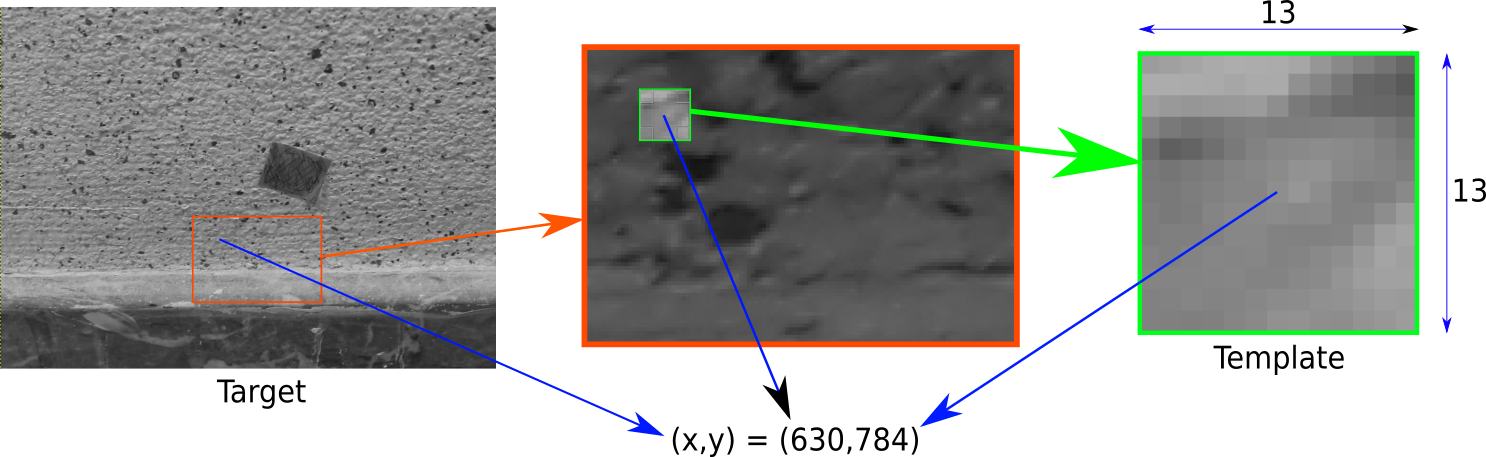
\includegraphics[width=15cm]{template_target.png}
\caption{Template taken from image (target) and ground truth position}
\label{fig:1.1}
\end{figure}

Our algorithm is:
\begin{itemize}
  \item Using correlation to quick localize potential image patch position.
  \item Using LSQ Matching to refine correlation result.
\end{itemize}


Because the template is taken directly from image, there isn't affinity between them. Hence, our LSQ model is taken from equation \ref{eq:2.6} without the affinity parameters. 

\begin{equation} 
\begin{aligned}
g_1(x_1,y_1) & = A*g_2(x_2,y_2) + B \\
 			 & \sim A*g_2(x_2,y_2) + B + g_2(x_2,y_2)*dA + A*(dg_2(x_2,y_2)) + dB \\
			 & = A*g_2(x_2,y_2) + B + g_2(x_2,y_2)*dA + A*(dg_2(Tr_x, Tr_y))\\
			 & 
			 + dB \\
			 & = A*g_2(x_2,y_2) + B + g_2(x_2,y_2)*dA \\
			 &
			 + A*(\frac{\partial g_2}{\partial x_2})*dTr_x 
			 + A*(\frac{\partial g_2}{\partial y_2})*dTr_y  \\
			 &
			 + dB
\end{aligned}
\end{equation}

\begin{equation} 
\begin{aligned}
		\Longrightarrow	 A*(\frac{\partial g_2}{\partial x_2})*dTr_x 
			 + A*(\frac{\partial g_2}{\partial y_2})*dTr_y
			 + dB
			 = g_1(x_1,y_1)-A*g_2(x_2,y_2)-B
\end{aligned}
\end{equation}

4 parameters to estimate : $d_{Tr_x}, d_{Tr_y}, d_{A}, d_{B}$.

This example program is implemented in \textit{"micmac/src/TpMMPD/Ex\_Match"}. There are 2 sources files and 1 header file:
\begin{itemize}
  \item cImgMatch.cpp
  \item cLSQTemplate.cpp
  \item cLSQTemplate.h
\end{itemize}
A source file {\color{blue}cImgMatch.cpp} contains constructor and methods \& for class {\color{blue}cImgMatch}. This class serve to describle an image. It also have methods to get an image patch from an image ({\color{orange}cImgMatch::GetImget}).

A source file {\color{blue}cLSQTemplate.cpp} contains constructor and methods \& for class {\color{blue}cLSQMatch}, function to compute correlation score, function to search best match position by correlation method \& the "main" function.

Let focus to the LSQ matching function in file {\color{blue}cLSQTemplate.cpp}. Function named {\color{orange}cLSQMatch::MatchbyLSQ} requires parameters as belown:
\begin{lstlisting}
bool cLSQMatch::MatchbyLSQ(
                           Pt2dr aPt1,			// an init point on image patch
                           const tIm2DM & aImg1,  // image patch                               
                           const tIm2DM & aImg2,  // image target
                           Pt2dr aPt2,			// an init point on image target
                           Pt2di aSzW,			// windows size
                           double aStep,			// pixel sampling step
                           Im1D_REAL8 & aSol		// LSQ result container
                          )
\end{lstlisting}

\begin{lstlisting}
{
    /*
     * Model : dA*g1 + dB + A*(dg2/dx)*dTrx + A*(dg2/dy)*dTrY = g1-A*g2-B (eq 1.15)
     */
    Pt2dr aPt(0,0);
    L2SysSurResol aSys(4);
    double mCoeff[4];
    // each couple of pixel correspondant in template & target is 1 observation
    for (aPt.x = -aSzW.x; aPt.x < aSzW.x; aPt.x = aPt.x + aStep)
    {
        for (aPt.y = -aSzW.y; aPt.y < aSzW.y; aPt.y = aPt.y + aStep)
        {
            Pt2dr aPC1 = aPt1 + aPt;
            Pt2dr aPC2 = aPt2 + aPt;
            // intensity value of pixel in template (g1)
            double aV1 = mInterpol->GetVal(aImg1.data(),aPC1);    
            Pt3dr aNewVD2= mInterpol->GetValDer(aImg2.data(),aPC2);   
            // derivation by X of g2
            double aGr2X = aNewVD2.x;  
		    // derivation by Y of g2
            double aGr2Y = aNewVD2.y;  
            // intensity value of pixel in target (g2)
            double aV2   = aNewVD2.z; 

	/* Fill up coefficient for each observation equation
	 * Notion in comment is correspondant with eq (1.15)    
	 */
            mCoeff[0] = aV1 ;  // g1 : coeff of dA
            mCoeff[1] = 1.0 ;  // coeff of dB
            mCoeff[2] = aGr2X; // coeff of dTrx
            mCoeff[3] = aGr2Y; // coeff of dTry
			
   // the right side of eq (1.15) is g1-A*g2-B, with A=1.0 & B=0.0 (init value)
            aSys.AddEquation(1.0,mCoeff,aV1-1.0*aV2-0.0); 
        }
    }
    /*==== This part of code adds a regulisation terms in LSQ system - it is optional
    double aReg=0.00001;
    for(int aK=0; aK<4; aK++)
    {
        aSys.AddTermQuad(aK,aK,aReg);
    }
    =================================================================================*/
    bool OK = false;
    aSol = aSys.Solve(&OK);
    return OK;
}
\end{lstlisting}

The program is implemented in command {\color{red}\textit{"mm3d TestLib LSQMatch"}}: 

\begin{verbatim}
*****************************
*  Help for Elise Arg main  *
*****************************
Mandatory unnamed args : 
  * string :: {Image Template}
  * string :: {Target Image to search for template}
Named args : 
  * [Name=Disp] bool :: {Display ? (click to Tar image)}
  * [Name=StepCor] REAL :: {Step of windows movement in Correlation}
  * [Name=StepPix] INT :: {Step of pixel sampling in 1 Correlation}
  * [Name=StepLSQ] REAL :: {Step of pixel sampling in LSQ}
  * [Name=NbIter] INT :: {Number of LSQ iteration (def=1)}
\end{verbatim}

Command parameter explication : 
\begin{itemize}
  \item Mandatory params:
  	\begin{itemize}
  		\item Image template (image patch to search for)
  		\item Image target (image to search for position of template)
  	\end{itemize}
  \item Optional params:
  	\begin{itemize}
  		\item \textit{\textbf{Disp}}: Display correlation windows step by step - (click in display windows to continue)
  		\item \textit{\textbf{StepCor}}: Foward step (in pixel) for each correlation window (same for X and Y).
  		\item \textit{\textbf{StepPix}}: Pixel sampling step in correlation. 
  		\item \textit{\textbf{StepLSQ}}: Pixel sampling step in LSQ
  		\item \textit{\textbf{NbIter}}: Number of iteration for LSQ refine matching. A new matched position is updated after each iteration as an initialization.
  	\end{itemize}
\end{itemize}

Now, execute the command as belown: 
\begin{verbatim}
mm3d TestLib LSQMatch Temp_13_Test.png Target.png StepCor=2.5 StepLSQ=0.5 NbIter=1
\end{verbatim}

$"Temp\_13\_Test.png"$ is template image patch extracted from image $"Target.png"$, with exact size and position as shown on \ref{fig:1.1}. \textit{StepCor=2.5} to speed up the correlation step (as it serve to initialize position for LSQ matching). The result shown:

\begin{verbatim}
Correl : 0.94847 - Pt: [629.5,784.5]
Create matching
In const cLSQMatch
==== Iter [0] =====
    **A: 0.0186942 -B: -3.50603 -TrX: 0.295016 -TrY: -0.285943
    **Before : [629.5,784.5] - After LSQ: [629.795,784.214]
\end{verbatim}

Here, correlation found that the best match position locates at $[629.5,784.5]$, and after refine this position by LSQ, it turns to $[629.795,784.214]$. If we compare with the ground truth (exact match position) $[630,784]$, LSQ is really help to approche better match location.

Can we do it better by adding more iteration on LSQ process ? Execute the command as belown:
\begin{verbatim}
mm3d TestLib LSQMatch Temp_13_Test.png Target.png StepCor=2.5 StepLSQ=0.5 NbIter=3
\end{verbatim}

The result shown:
\begin{verbatim}
Correl : 0.94847 - Pt: [629.5,784.5]
Create matching
In const cLSQMatch
==== Iter [0] =====
    **A: 0.0186942 -B: -3.50603 -TrX: 0.295016 -TrY: -0.285943
    **Before : [629.5,784.5] - After LSQ: [629.795,784.214]
==== Iter [1] =====
    **A: 0.00599393 -B: -1.16519 -TrX: 0.204943 -TrY: -0.212737
    **Before : [629.795,784.214] - After LSQ: [630,784.001]
==== Iter [2] =====
    **A: 4.19206e-09 -B: -8.2608e-07 -TrX: 4.12034e-05 -TrY: -0.00132025
    **Before : [630,784.001] - After LSQ: [630,784]
\end{verbatim}

The matching result of previous LSQ iteration is given as input for next LSQ iteration. Look how the matching position is better and better after each iteration. Finally, the exact match is founded at location $[630,784]$ at iteration 3.

\begin{figure}[h] 
\centering
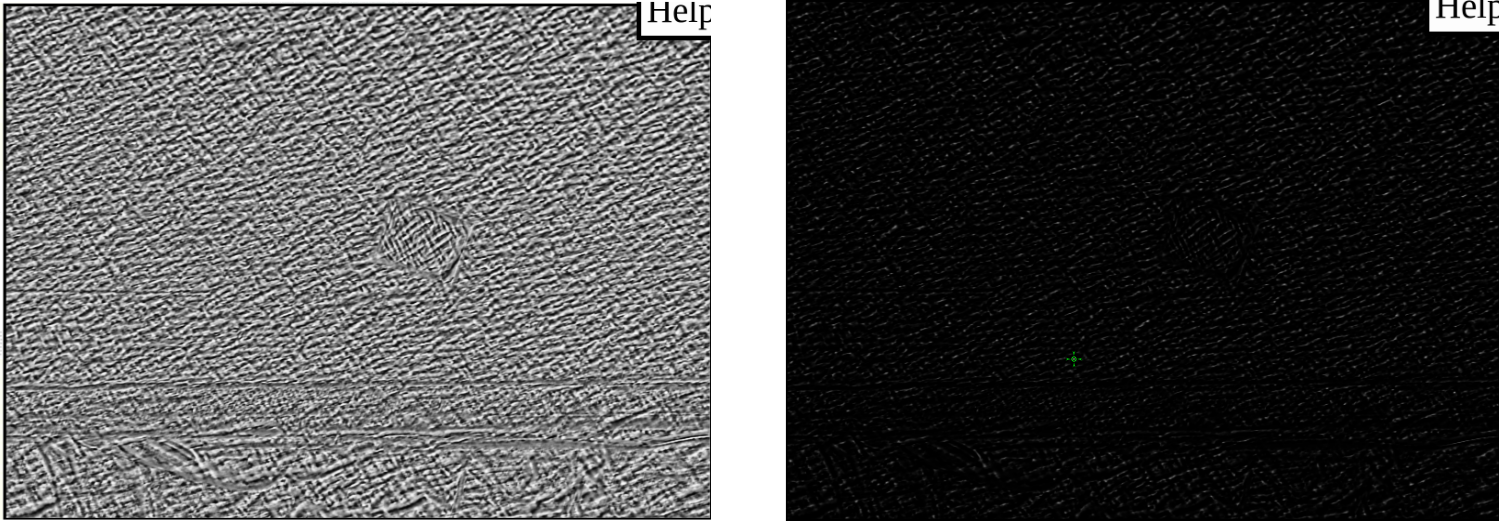
\includegraphics[width=12cm]{Correlation_img.png}
\caption{The correlation image shows best match position founded by correlation. (position marked by green circle in the right image (too hard to see because image is dynamic adaptation to show the pics of correlation, but trust me, it has plenty of white points :D ))}
\label{fig:1.2}
\end{figure}

\textbf{Example 2:} We have in this example a standard LSQ matching problem, with 8 parameters to estimate: 2 translation, 4 affinity, 2 radiometry. Our problem is described below: 

\begin{itemize}
  \item Take 2 image with different point of view (have affinity between them)
  \item Cut an template image patch on first image.
  \item Try to re-find the position of template image patch in second image (target). Estimate affinity between 2 image patch, then verify it by redressing 2 image patch in the same geometry.
\end{itemize}
\begin{figure}[h] 
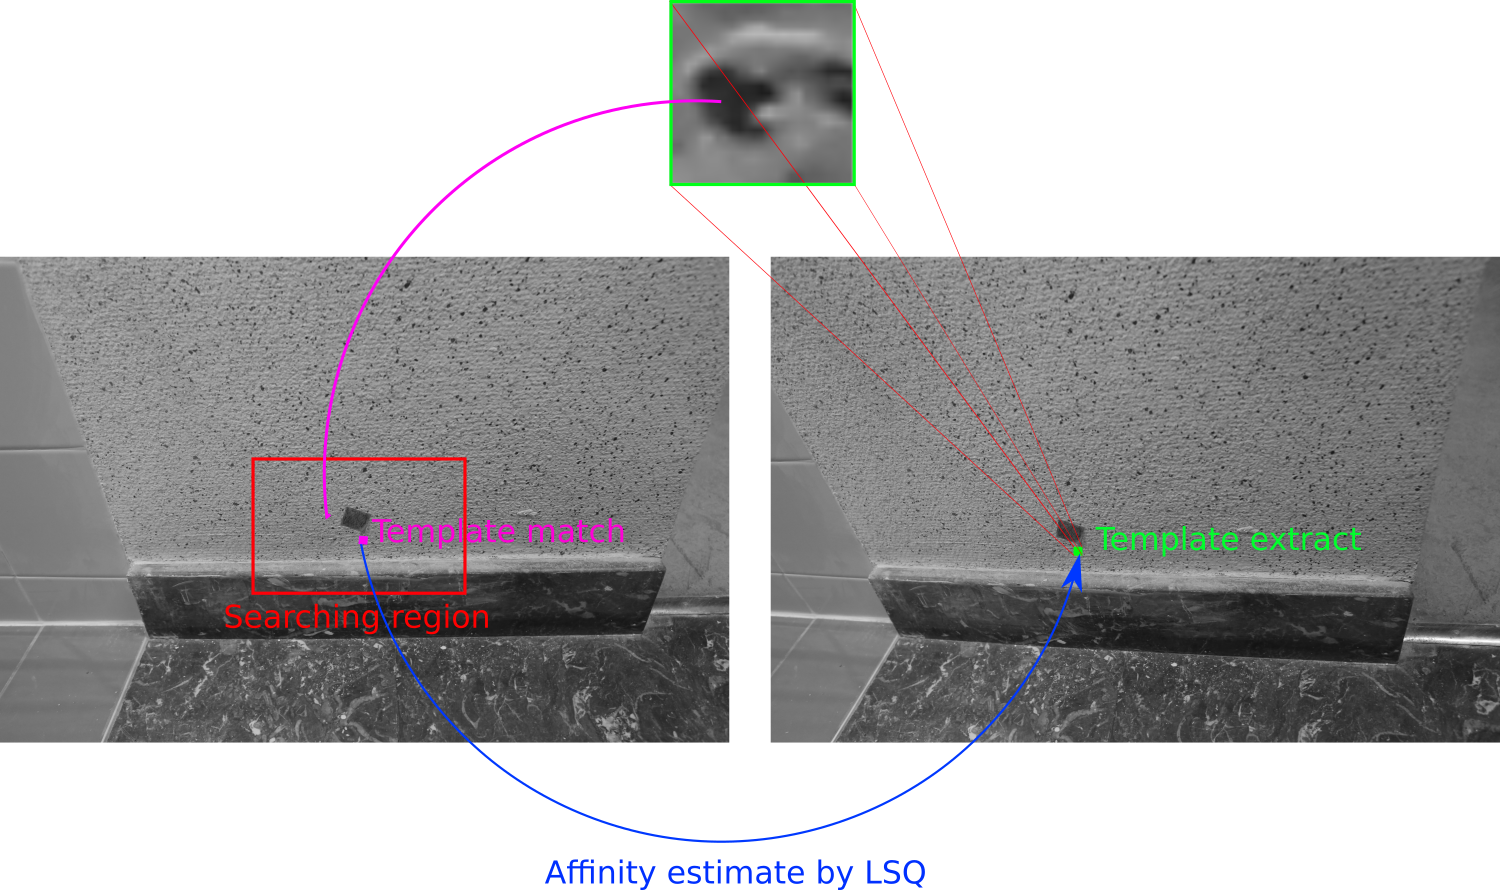
\includegraphics[width=15cm]{Matching_Temp_Ex2.png}
\caption{Example 2: Matching with template extracted from different point of view. (dataset used for this example also)}
\label{fig:2.3}
\end{figure}

As we seen on \ref{fig:2.3}, between the template (right image) and the target (left image), there are translation and affinity different.

Our algorithm is:
\begin{itemize}
  \item Using correlation to quick localize potential image patch position.
  \item Using LSQ Matching to refine correlation result by estimate translation and affinity between image patch.
\end{itemize}

Our LSQ model is taken from equation \ref{eq:2.6} with all of parameters liberated: 

$dA, dB, dTr_x, dTr_y, dAf10_x, dAf10_y, dAf01_x, dAf01_y$

In this code, we will write a program to do LSQ with the possibility of choosing number of parameters to be estimated. The code is written in {\color{blue}cLSQTemplate.cpp} - the "main" function. I will explain below the "most interesting" part of used to do LSQ:

\begin{lstlisting}
/*================= LSQ =====================*/
// Do refine matching by LSQ
aImgTarget->GetImget(aResCorrel.mPt, aImgTmplt->SzIm());
cLSQMatch * aMatch = new cLSQMatch(aImgTmplt, aImgTarget);
aMatch->Param() = aParam;

// Define number of variable to estimate
int aNbInconnu = 8;
// aParam.mCase is program entry parameter. User can choose which part to be estimated
switch (aParam.mCase)  
  {
    case 0: // estimate only 2 translation parameters
      {
        aNbInconnu = 2;	
        break;
      }
    case 1: // estimate 6 parameters: 2 translation + 4 affinity
      {
        aNbInconnu = 6;
        break;
      }
    case 2: // estimate 8 parameters: 2 translation + 4 affinity + 2 radiometry
      {
        aNbInconnu = 8;
        break;
      }
    case 3: // estimate 4 parameters: 2 translation + 2 radiometry 
      {
        aNbInconnu = 4;
        break;
      }
    case 4: // estimate 4 affinity parameters 
      {
        aNbInconnu = 4;
        break;
      }
  }

// variable initialization for LSQ
ElAffin2D aTransAffFinal(  Pt2dr(aResCorrelOrg.mPt - aPt1),
                           Pt2dr(1,0),
                           Pt2dr(0,1)
                        ); // Translation get value from correlation result
                           // Affinity get value identity (we don't have information before)
for (int aK=0; aK<aParam.mNbIter; aK++)
 {
  // for each iteration
  Im1D_REAL8 aSol(aNbInconnu); // contain estimated result	

  aMatch->MatchbyLSQ (
                       aPt1,                             // center point template image 
                       aImgTmplt->Im2D(),                // template image				
                       aImgTarget->Im2D(),               // target image
                       Pt2di(aImgTmplt->Im2D().sz()/2),  // size of region taken as observation on template image
                       aParam.mStepLSQ,                  // sampling pixel step for LSQ
                       aSol,                             // return result
                       aTransAffFinal                    // transformation from temp to target
                     );


  double * aResLSQ = aSol.data();
  // After estimation, we update our transformation from template to target:
  if (aParam.mCase == 0 || aParam.mCase == 3)    // trans only or Trans + Radio
  {
    cout<<"Delta: "<<Pt2dr(aResLSQ[0], aResLSQ[1])<<endl;
    // In case that we don't have affinity to estimate
    // => our transformation is update only with translation part
    aTransAffFinal = aTransAffFinal 
                     + ElAffin2D (  Pt2dr(aResLSQ[0],aResLSQ[1]),
                                    Pt2dr(0,0),
                                    Pt2dr(0,0)
                                 );
  }
  else
  {
    if (aParam.mCase == 4) 
    {
     // Affinity Only => only update affinity part
     aTransAffFinal = aTransAffFinal  + ElAffin2D(  Pt2dr(0,0),
                                                    Pt2dr(aResLSQ[0], aResLSQ[1]),
                                                    Pt2dr(aResLSQ[2], aResLSQ[3])
                                                 );
     }
     else
     {
      // Translation + affinity => update all part of transformation                    
      aTransAffFinal = aTransAffFinal  + ElAffin2D  ( Pt2dr(aResLSQ[0], aResLSQ[1]),
                                                      Pt2dr(aResLSQ[2], aResLSQ[3]),
                                                      Pt2dr(aResLSQ[4], aResLSQ[5])
                                                    );
     }
    }
  // this part for display result
  cout<<"==== Iter "<<"["<<aK<<"]"<<" ====="<<endl;
  cout<<"    ER **I00: "<< aTransAffFinal.I00() <<" -I01: "<< aTransAffFinal.I01() 
      <<" -I10: "<<aTransAffFinal.I10();
  
  if (aParam.mCase == 2)
    cout<<" -A: "<<aResLSQ[6]<<" -B: "<<aResLSQ[7];
  if (aParam.mCase == 3)
    cout<<" -A: "<<aResLSQ[2]<<" -B: "<<aResLSQ[3];
  cout<<endl;

  cout<<"    **Before : "<<aResCorrel.mPt;

  // update matching result
  aResCorrel.mPt = aTransAffFinal(aPt1);
  cout<<" - After LSQ: "<<aResCorrel.mPt<<endl<<endl;

 }
  // After all iteration, we have final estimate transformation
  cout<<"TransAff : "<<aTransAffFinal.I00()<<aTransAffFinal.I01()<<aTransAffFinal.I10()<<endl;
  cout<<endl<<endl;
\end{lstlisting}

As we seen, the code written in "main" function use to manage the iteration, update result...The function use to form the LSQ equation is written in {\color{blue}cLSQTemplate.cpp} - the {\color{blue}MatchbyLSQ} function: 

\begin{lstlisting}
bool cLSQMatch::MatchbyLSQ(
                                Pt2dr aPt1,
                                const tIm2DM & aImg1,   // template
                                const tIm2DM & aImg2,   // image
                                Pt2di aSzW,
                                double aStep,
                                Im1D_REAL8 & aSol,
                                ElAffin2D & aTrans12
                          )
{
    Pt2dr aPt(0,0);
    int aNbInconnu=8;
    switch (mParam.mCase)
    {
        case 0: // estimate only 2 translation parameters
            {
                aNbInconnu = 2;
                break;
            }
        case 1: // estimate 6 parameters: 2 translation + 4 affinity
            {
                aNbInconnu = 6;
                break;
            }
        case 2: // estimate 8 parameters: 2 translation + 4 affinity + 2 radiometry
            {
                aNbInconnu = 8;
                break;
            }
        case 3: // estimate 4 parameters: 2 translation + 2 radiometry 
            {
                aNbInconnu = 4;
                break;
            }
        case 4: // estimate 4 affinity parameters 
            {
                aNbInconnu = 4;
                break;
            }
    }
    L2SysSurResol aSys(aNbInconnu); //solveur declaration
    double mCoeff[8];
    double sqr_residu=0;
    for (aPt.x = -aSzW.x; aPt.x < aSzW.x; aPt.x = aPt.x + aStep)
    {
        for (aPt.y = -aSzW.y; aPt.y < aSzW.y; aPt.y = aPt.y + aStep)
        {
            // Scan through template patch
            Pt2dr aPC1 = aPt1 + aPt;
            // calcul position of correspondant pixel in target image by transformation given
            Pt2dr aPC2 = aTrans12(aPC1);
            // Get pixel value of correspondant pixel couple on 2 image patch
            double aV1 = mInterpol->GetVal(aImg1.data(),aPC1);    
            Pt3dr aNewVD2= mInterpol->GetValDer(aImg2.data(),aPC2);   
            double aGr2X = aNewVD2.x;  // derivation in X
            double aGr2Y = aNewVD2.y;  // derivation in Y
            double aV2   = aNewVD2.z;  // pixel intensity
            
            // this "switch" uses to form equation in each case of estimation.
            // These coefficient correspondant with equation (2.6)
            switch (mParam.mCase)
            {
                case 0: // only trans
                    {
                        mCoeff[0] = aGr2X ; // Trx
                        mCoeff[1] = aGr2Y ; // Try
                        break;
                    }
                case 1: // trans + Aff
                    {
                        mCoeff[0] = aGr2X ; // Trx
                        mCoeff[1] = aGr2Y ; // Try
                        mCoeff[2] = aGr2X*aPC1.x ; // im10
                        mCoeff[3] = aGr2Y*aPC1.x ;
                        mCoeff[4] = aGr2X*aPC1.y; // im01
                        mCoeff[5] = aGr2Y*aPC1.y;
                        break;
                    }
                case 2: // Trans + Aff + Radio
                    {
                        mCoeff[0] = aGr2X ; // Trx
                        mCoeff[1] = aGr2Y ; // Try
                        mCoeff[2] = aGr2X*aPC1.x ; // im10
                        mCoeff[3] = aGr2Y*aPC1.x ;
                        mCoeff[4] = aGr2X*aPC1.y; // im01
                        mCoeff[5] = aGr2Y*aPC1.y;
                        mCoeff[6] = aV2 ; // A
                        mCoeff[7] = 1.0 ; // B
                        break;
                        }
                case 3: // Trans + Radio
                    {
                        mCoeff[0] = aGr2X ; // Trx
                        mCoeff[1] = aGr2Y ; // Try
                        mCoeff[2] = aV2 ; // A
                        mCoeff[3] = 1.0 ; // B
                        break;
                    }
                case 4: // Aff
                    {
                        mCoeff[0] = aGr2X*aPC1.x ; // im10
                        mCoeff[1] = aGr2Y*aPC1.x ;
                        mCoeff[2] = aGr2X*aPC1.y; // im01
                        mCoeff[3] = aGr2Y*aPC1.y;
                        break;
                    }
            }
            aSys.AddEquation(1.0,mCoeff,aV1-aV2);
            sqr_residu+=(aV1-aV2)*(aV1-aV2);
        }
    }
    cout<<"sqr_residu: "<<sqrt(sqr_residu)<<endl;
    // ======= regulisation ====== //
    /*
    double aReg=0.0001;
    for(int aK=0; aK<aNbInconnu; aK++)
    {
        aSys.AddTermQuad(aK,aK,aReg);
    }
    */
    bool OK = false;
    aSol = aSys.Solve(&OK);
    cout<<"Retour solve: "<<OK<<endl;
    return OK;
}
\end{lstlisting}

Now, let see how this stuff works. The program is located in the same command with the example above: \textit{"mm3d TestLib LSQMatch"}:

\begin{verbatim}
*****************************
*  Help for Elise Arg main  *
*****************************
Mandatory unnamed args : 
  * string :: {Image Template}
  * string :: {Target Image to search for template}
Named args : 
  * [Name=Disp] bool :: {Display ? (click to Tar image)}
  * [Name=StepCor] REAL :: {Step of windows movement in Correlation}
  * [Name=StepPix] INT :: {Step of pixel sampling in 1 Correlation}
  * [Name=StepLSQ] REAL :: {Step of pixel sampling in LSQ}
  * [Name=NbIter] INT :: {Number of LSQ iteration (def=1)}
  * [Name=Case] INT :: {0 = Trans, 1 = Trans + Aff, 2 = Trans + Aff + Radio,  3 = Trans + Radio, 4 = Aff - def = 3}
  * [Name=Meth] INT :: {method corelation (0, 1=cCorrelImage)}
\end{verbatim}

There are two interesting optional parameters: \textbf{NbIter} use to define number of LSQ iteration and \textbf{Case} use to define which combination of parameters we want to estimate. We will analyse the method through these 2 parameters. Execute this command: 

\begin{verbatim}
mm3d TestLib LSQMatch template_c.tif b.tif StepCor=1 StepPix=1 StepLSQ=1 NbIter=10 Case=0 Meth=0
\end{verbatim}

This command search for template \textit{"template\_c.tif"} in target \textit{b.tif}
(dataset can be founded in Dataset folder). Correlation is done at entire pixel level (Zoom 1), LSQ sample pixel at entire level also (\textbf{StepLSQ=1}). (\textbf{Case=0}) mean that we just refine the translation part by LSQ. Let see the result:

\begin{verbatim}
Correlation Time : 8.7115
Correl : 0.929393 - Pt: [340,334]
Translation initiale: [328,322]

...
...
==== Iter [9] =====
    ER **I00: [327.726,322.265] -I01: [0,1] -I10: [1,0]
    **Before : [339.726,334.265] - After LSQ: [339.726,334.265]

TransAff : [327.726,322.265][0,1][1,0]
\end{verbatim}

We can see at the result that LSQ is refine the matching coordinate by translate matched point from $[340,334]$ to $[339.726,334.265]$. The final transformation from template patch to target patch given by LSQ is:
\begin{verbatim}
TransAff : [327.726,322.265][0,1][1,0]
\end{verbatim}
So, it is quite reasonable beacuse we don't estimate the affinity, so the affinity part in the transformation rest identical with value: $[0,1][1,0]$. We can verify the matching by apply this transformation in template image patch to recover the target patch and compare these 2:

\begin{figure}[h] 
\centering
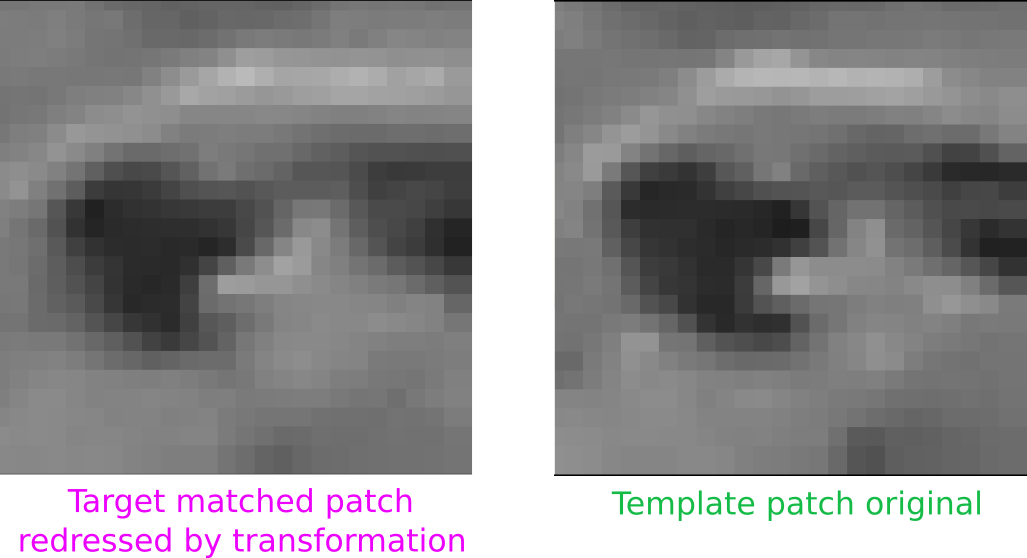
\includegraphics[width=10cm]{match_target_Trs.png}
\caption{Right: Template patch - Left: Target matched patch recover by transformation given by LSQ from template patch to target}
\label{fig:2.4}
\centering
\end{figure}

On the result Figure \ref{fig:2.4}, we can see that the matched patch is always display in his original geometry (of target image). This is normal because we just translate in image space of target image to find out the match.

Now, we can try to add the affinity part in the LSQ to estimate also:

\begin{verbatim}
mm3d TestLib LSQMatch template_c.tif b.tif StepCor=1 StepPix=1 StepLSQ=1 NbIter=10 Case=1 Meth=0
\end{verbatim}

Let see the result:
\begin{verbatim}
Correlation Time : 8.7496
Correl : 0.929393 - Pt: [340,334]
Translation initiale: [328,322]
...
...
==== Iter [9] =====
    ER **I00: [330.28,322.03] -I01: [-0.206441,1.03837] -I10: [1.01322,-0.0186548]
    **Before : [339.961,334.273] - After LSQ: [339.961,334.267]

TransAff : [330.28,322.03][-0.206441,1.03837][1.01322,-0.0186548]
\end{verbatim}

We can see that the affinity part is changed now. Transformation given by this process is:
\begin{verbatim}
TransAff : [327.726,322.265][0,1][1,0]
\end{verbatim}

Idem as above, apply this transformation to template patch to recover the matched patch to the same geometry, we obtain:

\begin{figure}[h] 
\centering
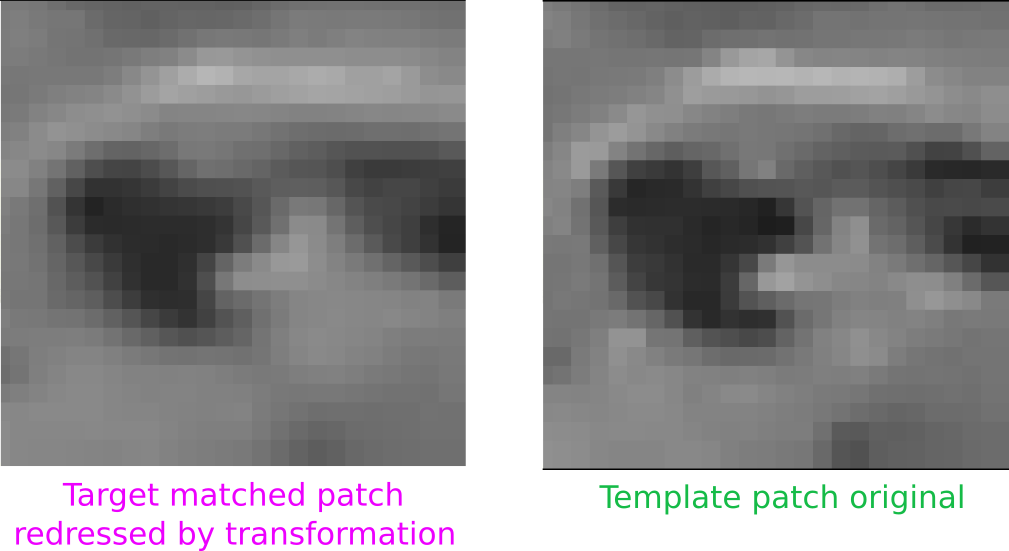
\includegraphics[width=10cm]{match_target_TrsAFF.png}
\caption{Right: Template patch - Left: Target matched patch recover by transformation given by LSQ from template patch to target}
\label{fig:2.4}
\centering
\end{figure}
We can see that the affine is estimated quite correct and it give a better result than LSQ matching with only translation estimate.

With this tutorial, I hope that you can using Least Square Solver module of MicMac for different purpose.

\end{document}





